%! Author = lazza
%! Date = 02/05/2022

\section{Hazards}\label{sec:hazards}
Dependencies are created at code-level and can be translated into conflicts when the compiler translate the code into
instructions.

A hazard is created whenever there is a conflict (and therefore a dependency) between instructions, and
these instructions are close enough that the overlap caused by pipelining would change the order of access to the
operands involved in the dependence.

Hazards prevent the next instruction in the pipeline from executing during its designated clock cycle, reducing the
performance from the ideal speedup gained by pipelining.

\subsection{Structural hazards}\label{subsec:structural-hazards}
Use of the same resource, such as the ALU, from different instructions simultaneously.
There cannot be structural hazards in the MIPS architecture:
\begin{description}
    \item[] Instruction Memory separated from Data Memory, thus allowing the fetch of instructions and the reading of
    register during the same clock cycle.
    \item[] Register File (RF) can be accessed twice in the same clock cycle: write access on the rising edge of
    the clock and read access on the falling edge by another instruction.
\end{description}

\subsection{Data Hazard}\label{subsec:data-hazard}
Attempt to use a result before it is ready, three different types:
\begin{itemize}
    \item[] RAW, read after write
    \item[] WAR, write after read
    \item[] WAW, write after write
\end{itemize}

\begin{figure}[h]
    \centering
    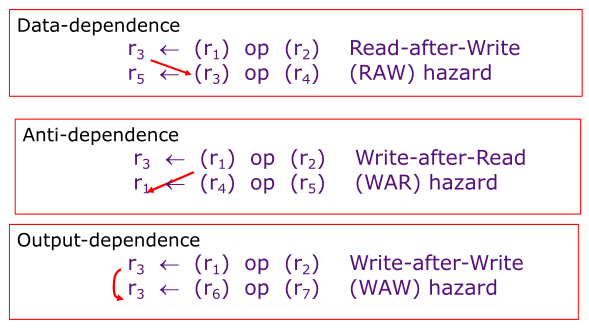
\includegraphics[scale = 0.4]{images/data-hazards-1}
    \caption{Data hazards}
    \label{fig:data-hazards}
\end{figure}


The RAW hazard is the only possible hazard in the MIPS architecture since all five stages are accessed in the
same order in and between instructions, this is due to the fact that in the MIPS architecture there cannot
be simultaneous or out-of-order access to the same resource.
The access to the resources follow the order of the instructions.

For this reason write backs are in-order and therefore WAW cannot happen, and the reading of registers of a previous
instruction happens always before the write back of a subsequent instruction precluding the WAR hazards.

In MIPS, RAW hazards can be dealt with at compile-time (design solution) or at run-time (hardware solution).

\paragraph{Compilation Techniques}
\begin{itemize}
    \item[\textrightarrow] Nop instructions, insertion of no operation
    \item[\textrightarrow] Instruction Scheduling, to avoid that correlating instructions are too close the compiler
    tries to insert independent instructions among correlated instructions.
\end{itemize}
Scheduling is a reordering of independent instructions without changing the overall result;
when the compiler does not find independent instructions, it inserts nops.

\paragraph{Hardware Techniques}
\begin{itemize}
    \item[\textrightarrow] Insertion of stalls (or bubbles) in the pipeline
    \item[\textrightarrow] Data Forwarding (or Bypassing)
\end{itemize}

Forwarding data means shortcutting data from one resource of the CPU, as output, to another resource of the CPU, as
input, using one clock cycle for the propagation, this means using temporary result stored in the pipeline instead of
waiting for the write back of results in the RF\@.
Forwarding costs are additional multiplexers to allow to fetch inputs from the pipeline.\\
In the MIPS architecture the common paths for data forwarding are EX-EX, MEM-EX, MEM-MEM\@.

Note that WB-ID is not a data path, data is written and accessed in the same clock cycle inside the Register File.
MEM-ID path is not useful if we divide clock cycle in rising and falling edge (optimized pipeline).


\begin{figure}[h]
    \centering
    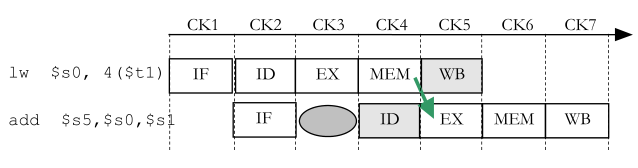
\includegraphics[scale=0.4]{images/load-use-hazard}
    \caption{Load/Use hazard requires a stall to use the MEM-EX path}
    \label{fig:load-use-hazard}
\end{figure}


\begin{figure}[h]
    \centering
    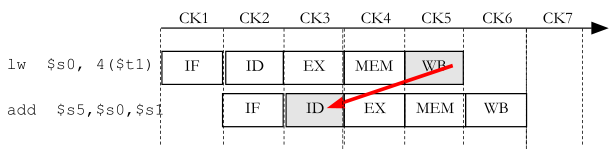
\includegraphics[scale=0.4]{images/load-use-without-forwarding}
    \caption{Load/Use without forwarding needs two stalls}
    \label{fig:load-use-without-forwarding}
\end{figure}


\begin{figure}[h]
    \centering
    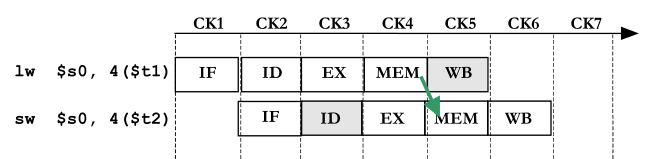
\includegraphics[scale=0.4]{images/load-store-hazard}
    \caption{Load/Store hazard uses the MEM-MEM path}
    \label{fig:load-store-hazard}
\end{figure}


\subsection{Control hazards}\label{subsec:control-hazards}
Attempt to make a decision on the next instruction to execute, before the condition is evaluated.
A MUX is responsible for the value of PC, which is based on ALU output: until the ALU doesn't evaluate the
condition the PC is not known, and we can't know which is the next instruction.

The PC is available at the MEM stage.

Generally true statements are executed in the waiting for the evaluation, as if the condition
were true and no jump was needed: just add to the PC plus one, and then see if the branch is taken.
For this particular reason it is suggested to write inside the \verb|IF| statements the code that most probably is
going to be executed.

In case we wait for the evaluation of the condition the stalls required are two in case of forwarding, three without forwarding.
%add figure explaing

An additional solution would be the early evaluation of the PC in the ID stage instead of the EXE stage, in this new
pipeline the PC adder is anticipated and only one stall would be required (with forwarding) to fetch the correct instruction.
This solution brings an issue in presence of a RAW hazard: anticipating the PC adder means that we have to add a stall
in order to solve the conflict.

\begin{figure}[h]
    \centering
    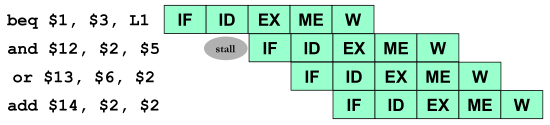
\includegraphics[scale = 0.4]{images/pc-early-evaluation}
    \caption{Early evaluation of the PC}
    \label{fig:pc-early-evaluation}
\end{figure}

\begin{figure}[h]
    \centering
    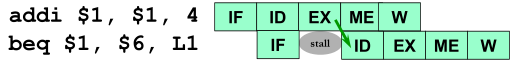
\includegraphics[scale = 0.4]{images/pc-early-evalutation-issue}
    \caption{PC early evaluation issue}
    \label{fig:pc-early-evaluation-issue}
\end{figure}